The user then clicks on  E21\_Person1 in the \rtworml mapping and selects Augment Data to discover new data to integrate into artist records.  
\karma retrieves \rtworml mappings in its repository that describe crm:E21\_Person, and uses these mappings to generate a candidate set of linked data sources to integrate, identifies meaningful object and data properties, and presents them to the user as illustrated in Figure~\ref{fig:search-screenshot}.
To help the users select properties to integrate, Karma uses Bloom filters to estimate the number of artists that have each of the properties listed in Figure~\ref{fig:search-screenshot}.
\begin{figure*}[t]
\centering
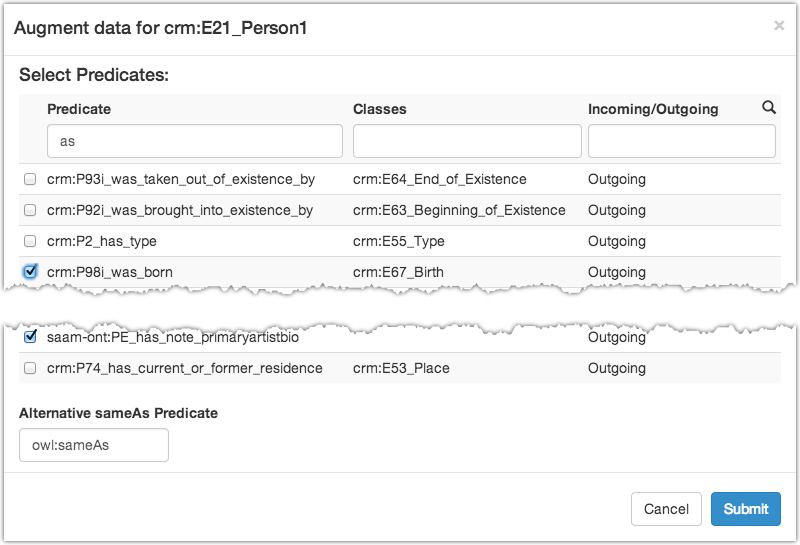
\includegraphics[width=4.9in]{images/5-search.png}
\vspace{-5mm}
\caption{A Karma user selects CIDOC CRM object and data properties discovered from other sources to augment crm:E21\_Person}
\vspace{-15pt}
\label{fig:search-screenshot}
\end{figure*}